% =====================================================================
% Section 5: Experimental Results (full section).
%   5.1  plausibility vs. grounding, human (RQ1)
%   5.2  observable vs. text-specified, human (RQ2)
%   5.3  failure cases (RQ3)
%   5.4  automated diagnosis (RQ4)            -- Som, with Aditya
% Tables in 5.3 are generated by backend/scripts/paper_tables.py;
% regenerate rather than hand-edit numbers. Self-contained: no \input.
% =====================================================================

\section{Experimental Results}
\label{sec:results}

This section presents results on the PhysicsLENS benchmark and evaluates its diagnostic pipeline through four research questions. RQ1--RQ3 are answered with human annotations, and RQ4 compares the pipeline against them. \textbf{RQ1:} Does high physical plausibility imply that a model followed a text-specified physical property (Sec.~\ref{sec:results-grounding})? \textbf{RQ2:} Does stating a property in text rather than showing it reduce physical plausibility (Sec.~\ref{sec:results-paired})? \textbf{RQ3:} What do individual failure cases reveal about the distinction between grounding and plausibility (Sec.~\ref{sec:results-cases})? \textbf{RQ4:} Can the PhysicsLENS pipeline approximate human judgments (Sec.~\ref{sec:results-tool})?

\subsection{RQ1: Does High Plausibility Imply Property Grounding?}
\label{sec:results-grounding}
A video can look physically realistic and still ignore the physics it was asked to show. Annotators rate each video's physical plausibility $P$ and, for unobservable videos, its adherence $H$ to the stated property, both on a 1--4 scale (Section~\ref{sec:human-annotation}): $P \geq 3$ means the video is mostly or fully physically realistic, and $H \leq 2$ means the stated property is mostly or completely ignored. Of the 119 unobservable videos, 47 are rated plausible ($P \geq 3$), yet 34 of these (72\%) ignore the stated property ($H \leq 2$). All four generators produce such videos (Table~\ref{tab:hidden-results}, Figure~\ref{fig:joint-ratings}). MAGI contributes 21 of the 34, but the pattern does not depend on it: without MAGI, 13 of the remaining 26 plausible videos (50\%) still ignore the property.

% Table 4 and Figure 4 side by side, top and bottom aligned: the plot's height
% is set to (table + its caption) - (figure caption), so both columns end together.
\newsavebox{\PLtab}\newsavebox{\PLcap}
\begin{figure}[t]
    \centering
    \sbox{\PLtab}{\begin{minipage}[t]{0.52\linewidth}
        \vspace{0pt}
        \centering
        \setlength{\abovecaptionskip}{0pt}
        \captionof{table}{Human evaluation on unobservable scenarios. $\bar{P}$, $\bar{H}$: mean plausibility and adherence (1--4). Compl.: completion rate.}
        \label{tab:hidden-results}
        \footnotesize
        \setlength{\tabcolsep}{2pt}
        \resizebox{\linewidth}{!}{%
        \begin{tabular}{@{}l r r r r r@{}}
            \toprule
            Model & $n$ & $\bar{P}$ & $\bar{H}$ & Compl. & $H{\le}2 \mid P{\ge}3$ \\
            \midrule
            HunyuanVideo 1.5  & 29 & 2.24 & 2.24 & 72.4\% & 5/13 (38.5\%) \\
            MAGI 4.5B distill & 30 & 3.10 & 1.10 &  6.7\% & 21/21 (100\%) \\
            Wan 2.2           & 30 & 1.53 & 1.90 & 40.0\% & 2/5 (40.0\%) \\
            Cosmos-nano 1     & 30 & 2.07 & 1.87 & 66.7\% & 6/8 (75.0\%) \\
            \bottomrule
        \end{tabular}}
    \end{minipage}}%
    \sbox{\PLcap}{\begin{minipage}[t]{0.45\linewidth}
        \vspace{0pt}
        \setlength{\abovecaptionskip}{4pt}
        \captionof{figure}{Mean plausibility ($P$) vs.\ mean adherence ($H$) per model (1--4).}
        \label{fig:joint-ratings}
    \end{minipage}}%
    \usebox{\PLtab}\hfill
    \begin{minipage}[t]{0.45\linewidth}
        \vspace{0pt}
        \centering
        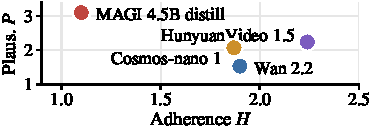
\includegraphics[width=\linewidth,
            height=\dimexpr\dp\PLtab-\dp\PLcap\relax]{fig/fig_mean_dotplot.pdf}\par\nointerlineskip
        \usebox{\PLcap}
    \end{minipage}
\end{figure}

The reverse also holds. Of the 28 videos that follow the stated property, 15 are rated implausible ($P \leq 2$): the model gets the property right but breaks other physics along the way. \textbf{Plausibility and grounding measure different things, and a benchmark has to measure both.}

\subsection{RQ2: Does Stating a Property in Text Reduce Plausibility?}
\label{sec:results-paired}

Each unobservable video has an observable twin: the same scene, action and generator, differing only in whether the property is shown in the image or stated in the text. Comparing twins, plausibility drops for every one of the four models when the property moves into the text, by 0.13 to 0.38 points on the 1--4 scale (Table~\ref{tab:paired-results}). Across all pairs, plausibility falls in 40 and rises in only 26.

% Table 5 and Figure 5 side by side, heights matched as for Table 4 / Figure 4.
\begin{figure}[t]
    \centering
    \sbox{\PLtab}{\begin{minipage}[t]{0.485\linewidth}
        \vspace{0pt}
        \centering
        \setlength{\abovecaptionskip}{0pt}
        \captionof{table}{Matched plausibility comparison. Obs., Unobs.: mean $P$ on the matched pairs; $\Delta$: unobservable minus observable. $p$: Holm-adjusted paired test; pooled row: scenario-level sign-flip test over the 29 scenarios annotated for all four models.}
        \label{tab:paired-results}
        \footnotesize
        \setlength{\tabcolsep}{3pt}
        \resizebox{\linewidth}{!}{%
        \begin{tabular}{@{}lrrrrr@{}}
            \toprule
            Model & $n$ & Obs. & Unobs. & $\Delta$ & $p$ \\
            \midrule
            HunyuanVideo 1.5  & 29 & 2.62 & 2.24 & $-0.38$ & 0.709 \\
            MAGI 4.5B distill & 30 & 3.33 & 3.10 & $-0.23$ & 0.884 \\
            Wan 2.2           & 30 & 1.83 & 1.53 & $-0.30$ & 0.497 \\
            Cosmos-nano 1     & 30 & 2.20 & 2.07 & $-0.13$ & 0.884 \\
            \midrule
            Pooled            & 29 & ---  & ---  & $-0.28$ & 0.085 \\
            \bottomrule
        \end{tabular}}
    \end{minipage}}%
    \sbox{\PLcap}{\begin{minipage}[t]{0.485\linewidth}
        \vspace{0pt}
        \setlength{\abovecaptionskip}{4pt}
        \captionof{figure}{Paired change $\Delta = P^{\mathrm{unobs}} - P^{\mathrm{obs}}$ per model and pooled, with bootstrap intervals over scenarios.}
        \label{fig:paired-effects}
    \end{minipage}}%
    \usebox{\PLtab}\hfill
    \begin{minipage}[t]{0.485\linewidth}
        \vspace{0pt}
        \centering
        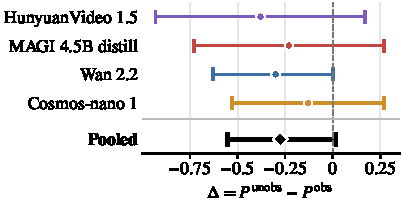
\includegraphics[width=\linewidth,
            height=\dimexpr\dp\PLtab-\dp\PLcap\relax]{fig/fig_forest_plausibility.pdf}\par\nointerlineskip
        \usebox{\PLcap}
    \end{minipage}
\end{figure}

Pooling the 29 scenarios that all four models generated gives the same picture: plausibility falls by 0.28 points on average (Figure~\ref{fig:paired-effects}; $p = 0.085$), and every model's estimate lies below zero. \textbf{Models produce less convincing physics when they have to read a property rather than see it.}

\subsection{RQ3: What Do Failure Cases Reveal About Grounding and Plausibility?}
\label{sec:results-cases}

\begin{figure}[t]
    \centering
    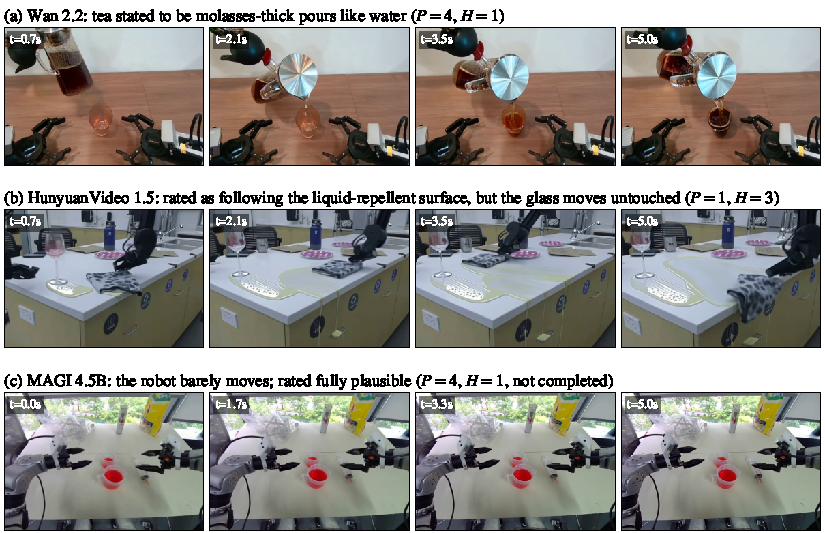
\includegraphics[width=\linewidth]{fig/fig_failure_cases.pdf}
    \caption{Three annotated failure cases (four frames each). $P$: physical plausibility; $H$: hidden-property adherence (both 1--4). (a) A clean, realistic pour that ignores the stated viscosity. (b) A video rated as following the stated property that is nevertheless physically implausible. (c) A nearly static video rated fully plausible.}
    \label{fig:failure-cases}
\end{figure}

Individual videos show how plausibility and grounding come apart (Figure~\ref{fig:failure-cases}; quotes are from the annotators' notes). In scenario 019, the prompt describes the tea as ``molasses-like'', yet all four models pour it like water ($H{=}1$) in videos rated realistic, and Wan~2.2 (Figure~\ref{fig:failure-cases}a) even receives the top plausibility rating: the models follow what the teapot looks like, not what the text says. The reverse also happens. In scenario 022, HunyuanVideo~1.5 follows the stated silicone-coated table ($H{=}3$) but is rated least plausible because of ``the glass moving without being touched'' (Figure~\ref{fig:failure-cases}b), and in scenario 070, Wan~2.2 keeps an ``extremely heavy'' tape dispenser still only because ``the robot's hand passes through it'' ($P{=}1$). MAGI's high plausibility often comes from inaction: in scenario 011 (Figure~\ref{fig:failure-cases}c) the robot barely moves, so nothing breaks physics because nothing happens. PhysicsLENS catches the visible failures, ranking HunyuanVideo's moving glass among the four least plausible of 433 videos and naming it a fluid violation with probability 0.997, as the annotators did, whereas the ignored viscosity in scenario 019 leaves nothing visibly wrong for any plausibility judge to catch. \textbf{Grounding has to be tested directly, and the matched design of PhysicsLENS makes that possible.}

\subsection{RQ4: Can PhysicsLENS Approximate Human Judgments?}
\label{sec:results-tool}

Can PhysicsLENS stand in for human annotators? We run its stages on all 439 annotated videos and compare the results with the human ratings, using ten open-weight VLMs from seven families (7B--32B parameters; Qwen3-VL, Qwen2.5-VL, InternVL3, Gemma-3, Llama-4-Scout, LLaVA-OneVision and Mistral-Small-3.1) and VideoPhy-2~\citep{bansal2026videophy} as an independent check. Each VLM answer is read as a probability; VLM answers and Stage-1/2 signals are combined with a weight fitted on the training folds, and any signal selection uses five-fold cross-validation that keeps every version of a scenario in the same fold, so nothing is tuned on the videos it is tested on. We report AUC: the probability that a better-rated video receives the higher score (0.5 is chance, 1 is perfect). Appendix~\ref{app:additional-results} gives the stage-by-stage results and agreement on the annotators' own scale.

\textbf{PhysicsLENS is the strongest evaluator.} Table~\ref{tab:main-results} compares PhysicsLENS with two baselines and with single VLM judges. The full system, which asks every question of all ten VLMs, averages their answers and combines them with the Stage-1/2 signals, is the best or tied-best system on six of the seven measures: plausibility (0.72 overall), task completion (0.81), violation detection (0.73), physics family (0.62) and property adherence (0.71). Even with a single VLM, adding PhysicsLENS evidence helps across the board: averaged over the ten VLMs, plausibility rises from 0.53 to 0.61, violation detection from 0.58 to 0.72, task completion from 0.71 to 0.76 and property adherence from 0.57 to 0.70, and detection and adherence improve for every one of the ten. The signals alone, with no VLM, already reach 0.70 on violation detection; the one selected most often measures objects vanishing mid-frame, a violation read directly off the tracker. The strongest baseline scores each video by its generator's average rating, which works because the four generators differ widely in quality. It ties PhysicsLENS on unobservable videos (0.72 vs.\ 0.71), but it cannot tell a good video from a bad one made by the same model: within each generator it scores 0.5 by construction, while PhysicsLENS reaches 0.67 on unobservable plausibility and 0.76 on task completion. It also does not exist for a new generator, which is exactly where an automatic evaluator is needed.

\begin{table*}[t]
    \centering
    \small
    \setlength{\tabcolsep}{2.4pt}
    \begin{tabular}{@{}lccc|cccc@{}}
        \toprule
        & \multicolumn{3}{c|}{Physical plausibility} & Task & Violation & Constr. & Hidden \\
        System & Obs. & Unobs. & All & compl. & detection & family & property \\
        \midrule
        \multicolumn{8}{@{}l}{\emph{Baselines}} \\
        Generator identity & 0.63{\scriptsize$\pm$0.03} & \textbf{0.72{\scriptsize$\pm$0.05}} & 0.65{\scriptsize$\pm$0.03} & 0.72{\scriptsize$\pm$0.02} & \textbf{0.73{\scriptsize$\pm$0.03}} & 0.51{\scriptsize$\pm$0.02} & 0.68{\scriptsize$\pm$0.05} \\
        Signals only (no VLM) & 0.61{\scriptsize$\pm$0.03} & 0.65{\scriptsize$\pm$0.05} & 0.62{\scriptsize$\pm$0.03} & 0.70{\scriptsize$\pm$0.03} & 0.70{\scriptsize$\pm$0.03} & 0.51{\scriptsize$\pm$0.02} & 0.69{\scriptsize$\pm$0.05} \\
        \midrule
        \multicolumn{8}{@{}l}{\emph{One VLM (mean $\pm$ sd over 10 backbones)}} \\
        VLM only & 0.53{\scriptsize$\pm$0.06} & 0.53{\scriptsize$\pm$0.06} & 0.53{\scriptsize$\pm$0.05} & 0.71{\scriptsize$\pm$0.04} & 0.58{\scriptsize$\pm$0.08} & 0.59{\scriptsize$\pm$0.02} & 0.57{\scriptsize$\pm$0.03} \\
        VLM + signals & 0.60{\scriptsize$\pm$0.02} & 0.66{\scriptsize$\pm$0.01} & 0.61{\scriptsize$\pm$0.01} & 0.76{\scriptsize$\pm$0.02} & 0.72{\scriptsize$\pm$0.01} & 0.58{\scriptsize$\pm$0.02} & 0.70{\scriptsize$\pm$0.02} \\
        Debiased VLM & 0.64{\scriptsize$\pm$0.07} & 0.63{\scriptsize$\pm$0.04} & 0.63{\scriptsize$\pm$0.06} & 0.71{\scriptsize$\pm$0.04} & 0.58{\scriptsize$\pm$0.08} & 0.59{\scriptsize$\pm$0.02} & 0.57{\scriptsize$\pm$0.03} \\
        Debiased VLM + signals & 0.65{\scriptsize$\pm$0.05} & 0.67{\scriptsize$\pm$0.03} & 0.65{\scriptsize$\pm$0.04} & 0.76{\scriptsize$\pm$0.02} & 0.72{\scriptsize$\pm$0.01} & 0.58{\scriptsize$\pm$0.02} & 0.70{\scriptsize$\pm$0.02} \\
        \midrule
        \multicolumn{8}{@{}l}{\emph{PhysicsLENS with all ten VLMs}} \\
        Ensemble, debiased & \textbf{0.73{\scriptsize$\pm$0.03}} & 0.71{\scriptsize$\pm$0.05} & \textbf{0.72{\scriptsize$\pm$0.02}} & 0.77{\scriptsize$\pm$0.02} & 0.67{\scriptsize$\pm$0.03} & \textbf{0.63{\scriptsize$\pm$0.01}} & 0.59{\scriptsize$\pm$0.06} \\
        Ensemble + signals (full) & \textbf{0.73{\scriptsize$\pm$0.03}} & 0.71{\scriptsize$\pm$0.05} & \textbf{0.72{\scriptsize$\pm$0.02}} & \textbf{0.81{\scriptsize$\pm$0.02}} & \textbf{0.73{\scriptsize$\pm$0.03}} & 0.62{\scriptsize$\pm$0.02} & \textbf{0.71{\scriptsize$\pm$0.05}} \\
        \bottomrule
    \end{tabular}
    \caption{PhysicsLENS against human judgment (AUC; 439 videos). \emph{Plausibility}: human rating 3--4 vs.\ 1--2. \emph{Task compl.}: completed vs.\ not. \emph{Violation detection}: any recorded violation vs.\ none. \emph{Constr.\ family}: naming which physics family was violated. \emph{Hidden property}: whether the stated property was followed (unobservable videos). \emph{Signals}: PhysicsLENS Stage-1/2 measurements, combined with the VLM answers using a weight fitted on training folds; the full system also includes temporal-embedding signals. \emph{Debiased}: the PhysicsLENS physics-error question, which replaces only the plausibility question. \emph{Ensemble}: every question asked of all ten VLMs and their answers averaged by rank, with no backbone selected. \emph{Generator identity} scores each video by its generator's average on the training folds. $\pm$: sd across the ten VLMs for the one-VLM rows, bootstrap sd over videos otherwise. Bold: best in each column.}
    \label{tab:main-results}
\end{table*}

\textbf{Why a VLM alone falls short.} Asked plainly whether a video is physically plausible, most VLMs do little better than chance (AUC 0.45--0.63; Table~\ref{tab:backbones-obs-unobs}). Shown two videos of the same task, they even pick the less realistic one more often than not (Gemma-3-12B is right in only 36\% of 347 pairs), because they favor the video with more motion and more task progress: VLMs treat \emph{plausible} as \emph{successful}, the same trap MAGI's near-static videos expose from the human side (Section~\ref{sec:results-cases}).

\textbf{Asking about physics errors, not overall realism.} The PhysicsLENS screening question instead asks the VLM to count specific physics errors (objects passing through each other, appearing or vanishing, floating, changing shape impossibly, or moving untouched) and to ignore task success and the amount of motion; the tables call it the \emph{debiased} question. This one change improves eight of the ten VLMs, the best by 0.20 (Qwen3-VL-32B: 0.55 to 0.75; InternVL3-14B: 0.51 to 0.71). It carries over to VideoPhy-2, a benchmark it was not designed for, where it significantly improves all three VLMs we tested (Qwen3-VL-32B: 0.645 to 0.720). It also lets bigger models pull ahead: with the plain question the 14B and 32B models trail their 7B and 8B counterparts, and with the PhysicsLENS question they lead them.

\begin{table}[t]
    \centering
    \small
    \setlength{\tabcolsep}{3.5pt}
    \begin{tabular}{@{}lcccccc|c@{}}
        \toprule
        & \multicolumn{2}{c}{VLM, standard prompt} & \multicolumn{2}{c}{VLM, debiased} & \multicolumn{2}{c|}{Debiased + S1/2} & Hidden \\
        \cmidrule(lr){2-3}\cmidrule(lr){4-5}\cmidrule(lr){6-7}
        Backbone & Obs. & Unobs. & Obs. & Unobs. & Obs. & Unobs. & AUC \\
        \midrule
        Signals only (S1/2) & --- & --- & --- & --- & 0.61 & 0.65 & 0.69 \\
        Qwen3-VL-32B & 0.55 & 0.55 & 0.75 & 0.70 & 0.74 & 0.70 & 0.57 \\
        InternVL3-14B & 0.51 & 0.45 & 0.71 & 0.65 & 0.71 & 0.68 & 0.51 \\
        Qwen3-VL-8B & 0.54 & 0.58 & 0.68 & 0.69 & 0.68 & 0.71 & 0.56 \\
        Qwen2.5-VL-32B & 0.45 & 0.44 & 0.66 & 0.64 & 0.67 & 0.71 & 0.57 \\
        InternVL3-8B & 0.63 & 0.62 & 0.66 & 0.59 & 0.65 & 0.61 & 0.59 \\
        Llama-4-Scout-17B & 0.58 & 0.48 & 0.64 & 0.61 & 0.64 & 0.65 & 0.59 \\
        Qwen2.5-VL-7B & 0.45 & 0.54 & 0.61 & 0.64 & 0.63 & 0.67 & 0.55 \\
        Gemma-3-12B & 0.61 & 0.61 & 0.59 & 0.59 & 0.60 & 0.65 & 0.56 \\
        LLaVA-OV-7B & 0.47 & 0.54 & 0.54 & 0.62 & 0.59 & 0.66 & 0.61 \\
        Mistral-Small-3.1-24B & 0.53 & 0.54 & 0.53 & 0.58 & 0.58 & 0.66 & 0.56 \\
        \bottomrule
    \end{tabular}
    \caption{Plausibility AUC for each VLM on observable ($n{=}320$) and unobservable ($n{=}119$) videos: with a standard question, with the PhysicsLENS physics-error (debiased) question, and with that question combined with Stage-1/2 signals (S1/2). \emph{Hidden}: AUC for judging whether the stated property was followed.}
    \label{tab:backbones-obs-unobs}
\end{table}

\textbf{Observable versus unobservable videos.} PhysicsLENS judges plausibility almost as well when the property is stated in text as when it is visible (Qwen3-VL-32B: 0.70 vs.\ 0.75). Judging whether the stated property was actually followed is harder, and this is where the signals help most, raising AUC from 0.51--0.61 for VLMs alone to 0.70 on average and 0.74 at best.

\textbf{Which kind of physics failed.} PhysicsLENS reliably detects each of the seven kinds of violation, separating affected videos from clean ones with AUC 0.66--0.84, and the signals improve this for six of the seven (Table~\ref{tab:category-accuracy}). Naming the exact family among several violations is harder, except for fluids (0.82): most violating videos (69\%) break several kinds of physics at once, and VLMs read frames largely one at a time, which suits single-frame failures such as a splash better than failures over time such as gravity or friction. Failures over time are exactly what the tracking-based measurements of the Stage-3 specialists are built for.

\begin{table}[t]
    \centering
    \small
    \setlength{\tabcolsep}{4pt}
    \begin{tabular}{@{}lrccc|cc@{}}
        \toprule
        & & \multicolumn{3}{c|}{Attribution AUC} & \multicolumn{2}{c}{Detection AUC} \\
        Constraint family & Pos. & Best VLM & Mean$\pm$sd (10) & Signals & Best VLM & +S1/2 \\
        \midrule
        Collision & 167 & 0.57 {\scriptsize Q3-32B} & 0.54$\pm$0.02 & 0.45 & 0.67 {\scriptsize Q3-32B} & 0.73 \\
        Deformation & 146 & 0.61 {\scriptsize G3-12B} & 0.58$\pm$0.03 & 0.60 & 0.68 {\scriptsize Q2.5-7B} & 0.74 \\
        Causality & 169 & 0.59 {\scriptsize Q3-32B} & 0.54$\pm$0.03 & 0.53 & 0.56 {\scriptsize Q3-8B} & 0.69 \\
        Momentum & 59 & 0.58 {\scriptsize Q2.5-7B} & 0.53$\pm$0.04 & 0.46 & 0.67 {\scriptsize Q3-8B} & 0.67 \\
        Gravity & 44 & 0.66 {\scriptsize Q2.5-7B} & 0.55$\pm$0.08 & 0.56 & 0.72 {\scriptsize Q3-8B} & 0.75 \\
        Fluid & 35 & 0.87 {\scriptsize Q2.5-7B} & 0.82$\pm$0.03 & 0.53 & 0.84 {\scriptsize Q2.5-7B} & 0.80 \\
        Friction & 24 & 0.65 {\scriptsize Q3-32B} & 0.57$\pm$0.05 & 0.48 & 0.66 {\scriptsize IV-14B} & 0.69 \\
        \bottomrule
    \end{tabular}
    \caption{Accuracy by physics family (AUC). \emph{Detection}: videos with this family vs.\ the 106 videos with no violation. \emph{Attribution}: videos with this family vs.\ videos with a different violation (Contact merged into Collision). \emph{Pos.}: videos with this family. \emph{Best VLM} is the best of ten; \emph{Mean$\pm$sd} is over all ten. Q3 = Qwen3-VL, Q2.5 = Qwen2.5-VL, IV = InternVL3, G3 = Gemma-3.}
    \label{tab:category-accuracy}
\end{table}

